\section{Anbringen von Henkeln}\label{sec:handle_attachment}
    Im Folgenden hei\ss e \({(x,y)\in\mathbb{D}^n}\) stets \({x\in\mathbb{D}^k}\) und \({y\in\mathbb{D}^k}\). Weiter sei zum Beispiel \({\mathbb{S}^{k-1}}\) durch \({\mathbb{S}^{k-1}\times\{0\}^{n-k}}\) als Untermannigfaltigkeit von \({\partial\mathbb{D}^n}\) aufgefasst.
    \subsection{Mannigfaltigkeiten mit Ecken}\label{subsec:manifolds_with_corners}
        Sei \({\mathcal{W}}\) eine glatte Mannigfaltigkeit mit Rand. Es kann die Mannigfaltigkeit mit Ecken \({H^k:=\mathbb{D}^k\times\mathbb{D}^{n-k}}\) betrachtet werden. Ihr Rand ist gerade
        \[\partial H^k=\mathbb{S}^{k-1}\times\mathbb{D}^{n-k}\cup\mathbb{D}^k\times\mathbb{S}^{n-k-1}\,,\]
        und l\"asst sich entlang einer Einbettung \({\Psi^k\colon\mathbb{S}^{k-1}\times\mathbb{D}^{n-k}\to\partial\mathcal{W}}\) zu dem topologischen Raum
        \[\mathcal{W}\mathop{+}^{\Psi}H^k:=\left(\mathcal{W}\sqcup H^k\right)/\left(\forall p\in\mathbb{S}^{k-1}\times\mathbb{D}^{n-k}\colon p\sim\Psi(p)\right)\]
        verkleben. Dieser Raum ist zweitabz\"ahlbar, hausdorffsch und lokal euklidisch. Das Problem besteht darin, dass es sich hierbei nicht unbedingt um eine glatte Mannigfaltigkeit mit Rand handelt, sondern vielmehr um eine glatte Mannigfaltigkeit mit Ecken, was den gesamten Beweis in die Kategorie der Mannigfaltigkeiten mit Ecken verschiebt, was etwas l\"astig ist. Es ist m\"oglich, diese Ecken zu gl\"atten, also eine hom\"oomorphe glatte Mannigfaltigkeit mit Rand zu finden. Dies ist nicht trivial und die Existenz einer Gl\"attung m\"usste gezeigt werden, sowie dieser Umstand bei allen Beweisen beachtet werden. Abgesehen davon ist der Ansatz etwas intuitiver und in Abbildung \ref{fig:one_handle} dargestellt.
        
    \newpage
    \subsection{Randsumme mit der Einheitsscheibe}\label{subsec:boundary_connected_sum_with_unit_disc}
        Andererseits l\"asst sich das Anbringen eines Henkels als die Randsumme einer Mannigfaltigkeit mit der Einheitsscheibe beschreiben. Hierzu sei die Umgebung \({U:=\mathbb{D}^n\setminus\mathbb{D}^{n-k}}\) von \({\mathbb{S}^{k-1}}\) in \({\mathbb{D}^n}\) definiert. Diese ist das Bild einer geeigneten Tubenumgebung \({\Tilde{h}_1\colon E\times\mathbb{R}_{\geq0}\hookrightarrow\mathbb{D}^n}\) mit dem riemannschen Vektorb\"undel
        \[\pi\colon E\to\mathbb{S}^{k-1},\,(p,x)\mapsto p\]
        f\"ur \({E:=\mathbb{S}^{k-1}\times\mathbb{R}^{n-k}}\) (siehe Appendix \ref{app:sphere_tub_emb}). Unter dieser Einbettung ist \({\alpha:=\Tilde{h}_1\circ\alpha_E\circ\Tilde{h}_1^{-1}}\) gerade
        \[\alpha\colon U\setminus\mathbb{S}^{k-1}\to U\setminus\mathbb{S}^{k-1},\,(x,y)\mapsto\left(x\frac{\sqrt{1-\norm{x}^2}}{\norm{x}},y\frac{\norm{x}}{\sqrt{1-\norm{x}^2}}\right)\,.\]
        Die Einschr\"ankung von \(\Tilde{h}\) auf \(E\times\{0\}\) ein, ergibt eine Tubenumgebung \(h\) von \({\mathbb{S}^{k-1}}\) in \({\partial\mathbb{D}^n}\) mit dem Bild \({U\cap\partial\mathbb{D}^n}\). Sei eine Einbettung \({\psi^k\colon\mathbb{S}^{k-1}\hookrightarrow\partial\mathcal{W}}\) mit einer Fortsetzungen \({\Psi^k\colon U\cap\partial\mathbb{D}^n\hookrightarrow\partial\mathcal{W}}\) und einer weiteren Fortsetzung \({\Tilde{\Psi}^k\colon U\hookrightarrow\mathcal{W}}\) von \({\Psi^k}\) gegeben, kann die Tubenumgebung \({\Tilde{h}_2:=\Tilde{\Psi}\circ\Tilde{h}_1}\) von \({\Lambda^k:=\psi^k(\mathbb{S}^{k-1})}\) in \({\mathcal{W}}\), und somit auch
        \[\mathcal{W}+\Psi^k:=\mathcal{W}\mathop{+}^{\mathbb{S}^{k-1}}\mathbb{D}^n\]
        definiert werden. In dieser gilt die Identifikation \({\Tilde{h}_1(x)\sim\Tilde{h}_2\circ\alpha_E(x)}\) f\"ur alle \({x\in E\times\mathbb{R}_{\geq0}\setminus\mathbf{0}}\), und wegen
        \[\Tilde{h}_2\circ\alpha_E(x)=\Tilde{\Psi}\circ\Tilde{h}_1\circ\Tilde{h}_1^{-1}\circ\alpha\circ\Tilde{h}_1(x)=\Tilde{\Psi}\circ\alpha\circ\Tilde{h}_1(x)\]
        auch \({y\sim\Tilde{\Psi}\circ\alpha(y)}\) f\"ur \({y\in U\setminus\mathbb{S}^{k-1}}\). Folglich ist
        \[\mathcal{W}+\Psi^k=\left(\mathcal{W}\setminus\Lambda^k\sqcup\mathbb{D}^n\setminus\mathbb{S}^{k-1}\right)/\left(y\sim\Tilde{\Psi}\circ\alpha(y)\,,y\in U\setminus\mathbb{S}^{k-1}\right)\]
        und es muss nicht mehr mit den tats\"achlichen Tubenumgebungen gearbeitet werden. Ein Henkel sei das Tripel \({(\psi^k,\Psi^k,\Tilde{\Psi}^k)}\), welches auch mit \({\Psi^k}\) bezeichnet werde.
    
    \subsection{\"Aquivalenz der Ans\"atze}\label{rem:equiv_corners_boundary_sum}
        Die R\"aume aus den Abschnitten \ref{subsec:manifolds_with_corners} und \ref{subsec:boundary_connected_sum} sind zueinander ho\-m\"oo\-morph, sodass die zusammenh\"angende Summe entlang der eingebetteten Sph\"are im Rand als Gl\"at\-tung der oben diskutierten Mannigfaltigkeit mit Ecken angesehen werden kann. 
    
    \subsubsection{Notation}
        Sei \({\Psi^k}\) ein Henkel, so hei\ss e die durch \({\Psi^k}\) eingebettete Sph\"are \({\Lambda^k}\) die Anklebesph\"are von \({\Psi^k}\) und \({\Sigma^k:=\mathbb{S}^{n-k-1}}\) der G\"urtel von \({\Psi^k}\). Hierbei gilt die Beziehung \({\Sigma^k=\partial\left(\mathcal{W}+\Psi^k\right)\setminus\partial\mathcal{W}}\). Der Kern von \({\Psi^k}\) sei die abgeschlossene H\"ulle von \({\mathring{\mathbb{D}}^{n-k}}\) in \({\mathcal{W}+\Psi^k}\).
        
        \begin{figure}
            \centering
            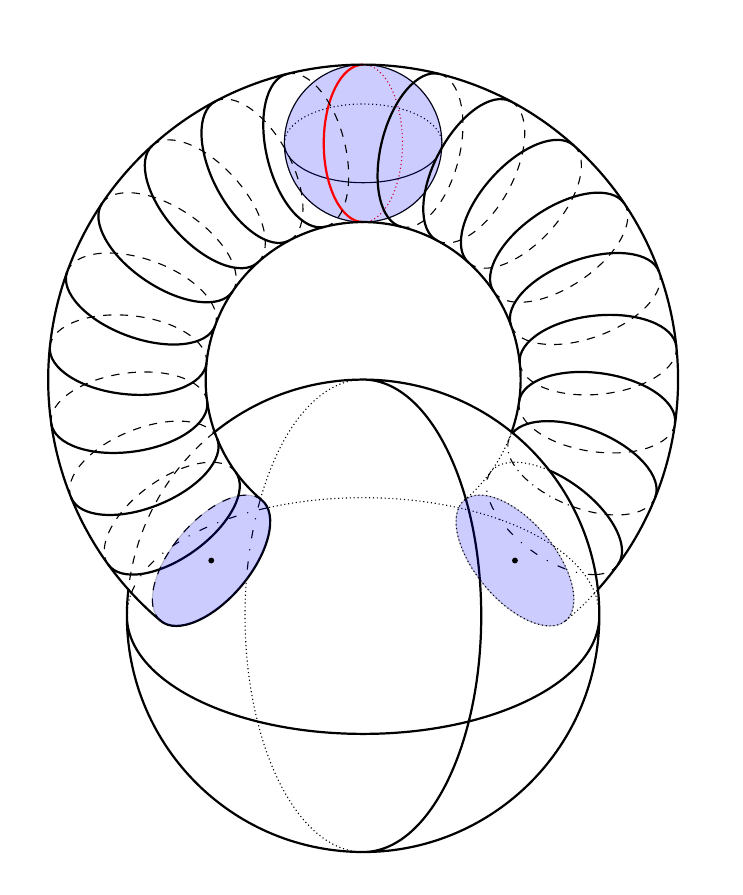
\begin{tikzpicture}
                \begin{scope}[yshift = 3cm] % Small ball
                    \draw [red, densely dotted]
                        (-90:0.5 and 1) arc (-90:90:0.5 and 1);
                    \draw
                        (1, 0) arc (0:360:1)
                        (180:1 and 0.5) arc (180:360:1 and 0.5);
                    \draw [densely dotted]
                        (0:1) arc (0:180:1 and 0.5);
                    \draw [fill = blue, opacity = 0.2] 
                        (1, 0) arc (0:360:1) -- cycle;
                    \draw [red, thick]
                        (90:0.5 and 1) arc (90:270:0.5 and 1);
                \end{scope}
                 %  Positions of circles
                \path[scale = 3] (-50:1) arc (-50:230:1)
                \foreach\i in {0, 0.05, 0.1, 0.15, 0.2, 0.25, 0.3, 0.35, 0.4, 0.45, 0.5, 0.55, 0.6, 0.65, 0.7, 0.75, 0.8, 0.85, 0.9, 0.95, 1} { node [pos = \i] (A\i) {}};
                % End of Tube
                \draw [thick]
                    (-41.75:4) arc (-41.75:230:4) 
                    (-19.5:2) arc (-19.5:230:2);
                \draw [densely dotted] 
                    (-50:4) arc (-50:-41.75:4) 
                    (-50:2) arc (-50:-19.5:2);
                % First circle
                \draw [densely dotted, rotate = -50] ({A0}.center) ++(0:1 and 0.5) arc (0:360:1 and 0.5);
                \begin{scope}[rotate = -36]     % Second circle
                    \draw [thick] ({A0.05}.center) ++(0:1 and 0.5) arc (0:114:1 and 0.5);
                    \draw [densely dotted] ({A0.05}.center) ++(115:1 and 0.5) arc (115:180:1 and 0.5);
                    \draw [loosely dashdotted] ({A0.05}.center) ++(-180:1 and 0.5) arc (-180:-32:1 and 0.5);
                    \draw [dashed] ({A0.05}.center) ++(-32:1 and 0.5) arc (-32:0:1 and 0.5);
                \end{scope}
                \begin{scope}[rotate = -22]     % Third circle
                    \draw [thick] ({A0.1}.center) ++(0:1 and 0.5) arc (0:170:1 and 0.5);
                    \draw [dashed] ({A0.1}.center) ++(-86:1 and 0.5) arc (-86:0:1 and 0.5);
                    \draw [densely dotted] ({A0.1}.center) ++(170:1 and 0.5) arc (170:180:1 and 0.5);
                    \draw [dashdotted] ({A0.1}.center) ++(180:1 and 0.5) arc (180:274:1 and 0.5);
                \end{scope}
                % Big ball
                \begin{scope}[yshift = -3cm, scale = 3]
                    \draw [thick]
                        (-186.5:1) arc (-186.5:129:1) 
                        (-90:0.5 and 1) arc (-90:90:0.5 and 1) 
                        (180:1 and 0.5) arc (180:360:1 and 0.5);
                    \draw [dashed]
                        (129:1) arc (129:173.5:1);
                    \draw [densely dotted]
                        (0:1 and 0.5) arc (0:114:1 and 0.5) 
                        (180:1 and 0.5) arc (180:169:1 and 0.5) 
                        (90:0.5 and 1) arc (90:150.5:0.5 and 1) 
                        (270:0.5 and 1) arc (270:171.25:0.5 and 1);
                    \draw [loosely dashdotted] 
                        (114:1 and 0.5) arc (114:169: 1 and 0.5)
                        (150.5:0.5 and 1) arc (150.5:171.25:0.5 and 1);
                \end{scope}
                % Remaining circles
                \foreach\i in {0.15, 0.2, 0.25, 0.3, 0.35, 0.4, 0.45, 0.55, 0.6, 0.65, 0.7, 0.75, 0.8, 0.85, 0.9, 0.95, 1} {
                    \begin{scope} [rotate = -50 + \i * 280]
                        \draw [thick] ({A\i}.center) ++(0:1 and 0.5) arc (0:180:1 and 0.5);
                        \draw [dashed] ({A\i}.center) ++(180:1 and 0.5) arc (180:360:1 and 0.5);
                    \end{scope}
                }
                % Attaching-Spheres
                \draw [fill = blue, opacity = 0.2, rotate = 230] 
                    ({A1}.center) ++(0:1 and 0.5) arc (0:360:1 and 0.5);
                \draw [fill = blue, opacity = 0.2, rotate = -50] 
                    ({A0}.center) ++(0:1 and 0.5) arc (0:360:1 and 0.5);
                \draw 
                    ({A1}.center) node [circle, fill, inner sep=0.75pt] {}
                    ({A0}.center) node [circle, fill, inner sep=0.75pt] {};
            \end{tikzpicture}
            \caption{Eine 3-Vollkugel mit einem 1-Henkel, die gleichzeitig eine optische T\"auschung ist. Dies ist hom\"oomorph zu einem Torus, also einem Diskb\"undel des Ranges \({2}\) \"uber der \({1}\)-Sph\"are (siehe Bemerkung \ref{rem:equiv_corners_boundary_sum} und Lemma \ref{lem:glueing_disc_bundles}).}\label{fig:one_handle}
        \end{figure}
    
    \newpage
    \begin{lemma}[Henkel an der Einheitskugel]\label{lem:handle_on_unit_disc}
        Das Anbringen eines Henkels an \({\mathbb{D}^n}\) entlang \({\mathbb{S}^{k-1}}\) ist zu einem Schei\-ben\-b\"un\-del des Ranges \({n-k}\) diffeomorph.
    \end{lemma}
    \begin{proof}
        Sei die Anklebeabbildung durch \({\psi^k\colon\mathbb{S}_1^{k-1}\to\mathbb{S}_2^{k-1}}\) gegeben. Eine m\"ogliche Fortsetzung von dieser ist
        \[\dot{\Psi}^k\colon U_1\cap\partial\mathbb{D}_1^n\to U_2\cap\partial\mathbb{D}_2^n,\,(x,y)\mapsto\left(\norm{x}\psi^k\left(\frac{x}{\norm{x}}\right),y\right)\,.\]
        Sei \({\ddot{\Psi}^k\colon U_1\cap\partial\mathbb{D}_1^n\to U_2\cap\partial\mathbb{D}_2^n}\) eine weitere, beliebige Fortsetzung von \({\psi^k}\). Dann sind die zugeh\"origen Tubenumgebungen von \({\mathbb{S}_2^{k-1}}\) in \({\partial\mathbb{D}_2^n}\) gerade
        \[\dot{h}_2=\dot{\Psi}^k\circ h_1\quad\text{und}\quad\ddot{h}_2=\ddot{\Psi}^k\circ h_1\,,\]
        und es existiert eine Isometrie, sodass \({\ddot{h}_2\simeq\dot{h}_2\circ\Gamma}\), und somit auch
        \[\ddot{\Psi}^k=\ddot{h}_2\circ h^{-1}\simeq\dot{h}_2\circ\Gamma\circ h_1^{-1}=\dot{\Psi}^k\circ h_1\circ\Gamma\circ h_1^{-1}\]
        gilt. Hierbei existiert eine glatte Abbildung \({\gamma\colon\mathbb{S}_1^{k-1}\to O\left(n-k\right)}\), sodass
        \[h_1\circ\Gamma\circ h_1^{-1}(x,y)=\left(x,\gamma\left(\frac{x}{\norm{x}}\right)\cdot y\right)\]
        ist. Folglich kann als Fortsetzung stets \({\Psi^k:=\dot{\Psi}^k\circ h_1\circ\Gamma\circ h_1^{-1}}\) gew\"ahlt werden, f\"ur welche
        \[\Psi(x,y)=\left(\norm{x}\psi^k\left(\frac{x}{\norm{x}}\right),\gamma\left(\frac{x}{\norm{x}}\right)\cdot y\right)\]
        gilt. Eine Fortsetzung dieser ist
        \[\Tilde{\Psi}^k\colon U_1\to U_2,\,z\mapsto\norm{z}\Psi^k\left(\frac{z}{\norm{z}}\right)\,.\]
        Diese Konstruktion ergibt nun
        \[\mathbb{D}^n+\Psi^k=\left(\mathbb{D}_1^n\setminus\mathbb{S}_1^{k-1}\right)\sqcup\left(\mathbb{D}_2^n\setminus\mathbb{S}_2^{k-1}\right)/\left(z\sim\Tilde{\Psi}^k\circ\alpha(z)\right)\]
        und besitzt die Untermannigfaltigkeit
        \[\mathcal{M}:=\mathring{\mathbb{D}}_1^k\sqcup\mathring{\mathbb{D}}_2^k/\left(x\sim\Tilde{\Psi}^k\circ\alpha(x)\right)\,,\]
        die zu der \({k}\)-Sph\"are hom\"oomorph ist (!). Es l\"asst sich nachrechnen, dass diese Identifikationen mit der Projektion
        \[\mathbb{D}^n+\Psi^k\to\mathcal{M},\,(x,y)\mapsto x\]
        kommutieren (siehe Appendix \ref{app:disc_bundle_well_defined}), sodass sich eine Faserb\"undelstruktur ergibt, deren Fasern diffeomorph zu Scheiben sind.
    \end{proof}

    \newpage
    \section{Vertauschung der Befestigungsreihenfolge}
        \begin{lemma}[Sortierungs-Lemma]\label{lem:sort_handles}
            Sei \({\mathcal{W}^n}\) ein Kobordismus und
            \[\Psi^i\colon\mathbb{S}^{i-1}\to\partial_+\mathcal{W}\quad\text{sowie}\quad\Psi^j\colon\mathbb{S}^{j-1}\to\partial_+\left(\mathcal{W}+\Psi^i\right)\]
            Henkel mit \({j\leq i\leq n}\). Dann existiert ein in \({\partial_+\left(\mathcal{W}+\Psi^i\right)}\) zu \({\Psi^j}\) iso\-to\-
            per Henkel \({\Phi^j\colon\mathbb{S}^{j-1}\to\partial_+\mathcal{W}}\) derart, dass
            \[\left(\mathcal{W}+\Psi^i\right)+\Psi^j\cong\left(\mathcal{W}+\Phi^j\right)+\Psi^i\,.\]
        \end{lemma}
        \begin{proof}
            Der Henkel \({\Psi^j}\) ist isotop zu einem Henkel dessen Anklebesph\"are \({\Lambda^j}\) den G\"urtel von \({\Psi^i}\) transversal schneide. Da die Anklebesph\"are die Dimension \({j-1}\), und der G\"urtel die Dimension \({n-i-1}\) besitzt, kann die Dimension der Summe der Tangentialvektorr\"aume in allen Schnittpunkten h\"ochstens
            \[(j-1)+(n-i-1)\leq n-2<n-1=\dim\partial_+\mathcal{W}\]
            betragen, sodass Transversalit\"at nur im trivialen Fall gegeben sein kann, also wenn der Schnitt leer ist. Ist die Anklebesph\"are jedoch disjunkt von dem G\"urtel von \({\Psi^i}\), so liegt diese per Definitionem bereits komplett in \({\partial_+\mathcal{W}}\). Jede Tubenumgebung von \({\Lambda^j}\) kann durch eine weitere Isotopie derart geschrumpft werden, dass diese ebenso komplett in \({\partial_+\mathcal{W}\setminus\Lambda^i}\) liegt. Das Anbringen des resultierenden Henkels \({\Phi^j}\) ist nun nicht mehr von \({\Psi^i}\) abh\"angig, sodass die Reihenfolge vertauscht werden kann.
        \end{proof}

        \subsection{Allgemeine Vertauschung}
            Sei \({\mathcal{W}}\) ein Kobordismus. Liegen f\"ur \({1\leq j\leq l}\) Einbettungen 
            \[\Psi_j^k\colon\mathbb{S}^{k-1}\to\partial_+\left(\mathcal{W}+\Psi_1^k+\Psi_2^k+\dots+\Psi_{j-1}^k\right)\] 
            vor, so zeigt eine zu dem Beweis des Lemmas sehr \"ahnliche Argumentation, dass f\"ur jedes \({\Psi_j^k}\) eine isotope Einbettung
            \[\Phi_j^k\colon\mathbb{S}^{k-1}\to\partial_+\mathcal{W}\]
            gefunden werden kann, deren Bild von allen anderen Anklebesph\"aren disjunkt ist. Insbesondere muss bis auf Diffeomorphie bei der Definition nicht auf die zuvor angebrachten Henkel geachtet werden. Dies rechtfertigt die Schreibweise
            \begin{align*}
                \mathcal{W}+\sum_{j=1}^l\Psi_j^k:&=\left(\dots\left(\left(\mathcal{W}+\Psi_1^k\right)+\Psi_2^k\right)+\dots\right)+\Psi_l^k\\
                &\cong\mathcal{W}+\Phi_1^k+\Phi_2^k+\dots+\Phi_l^k\,.
            \end{align*}

        \subsection{Henkelzerlegungen}
            Der Vertauschungssatz erm\"oglicht nun eine gezielte Definition einer Henkelzerlegung eines Kobordismus \({\left(\mathcal{W}^n,\mathcal{M},\mathcal{N}\right)}\).
            \begin{definition}[Henkelzerlegung]
                Eine Folge von Kobordismen \({\left(\mathcal{W}_k,\mathcal{M},\partial_+\mathcal{W}_k\right)}\) mit \({\mathcal{W}_{-1}=\mathcal{M}\times\mathbb{I}}\), \({\mathcal{W}_n\cong\mathcal{W}}\) und Zahlen \({p_k\in\mathbb{N}}\) f\"ur \({0\leq k\leq n}\), sowie Henkeln 
                \[\Phi_j^{k+1}\colon\mathbb{S}^k\to\partial_+\mathcal{W}_k\,,\quad\text{sodass}\quad\mathcal{W}_{k+1}\cong\mathcal{W}_k+\sum_{j=1}^{p_k}\Phi_j^{k+1}\]
                gilt und die Anklebesph\"aren aller \({\Phi_j^{k+1}}\) voneinander disjunkt seien.
            \end{definition}
            In der Anwendung des Sortierungs-Lemmas auf Henkel in einer Henkelzerlegung sei Obacht geboten. Durch die Diffeotopie werden auch m\"og\-lich\-er\-wei\-se die Anklebesph\"aren von sp\"ater angebrachten Henkeln verschoben.